% This is "sig-alternate.tex" V2.1 April 2013
% This file should be compiled with V2.5 of "sig-alternate.cls" May 2012
%
% This example file demonstrates the use of the 'sig-alternate.cls'
% V2.5 LaTeX2e document class file. It is for those submitting
% articles to ACM Conference Proceedings WHO DO NOT WISH TO
% STRICTLY ADHERE TO THE SIGS (PUBS-BOARD-ENDORSED) STYLE.
% The 'sig-alternate.cls' file will produce a similar-looking,
% albeit, 'tighter' paper resulting in, invariably, fewer pages.
% This .tex file (and associated .cls V2.5) produces:
%       1) The Permission Statement
%       2) The Conference (location) Info information
%       3) The Copyright Line with ACM data
%       4) NO page numbers
%
% as against the acm_proc_article-sp.cls file which
% DOES NOT produce 1) thru' 3) above.
%
% Using 'sig-alternate.cls' you have control, however, from within
% the source .tex file, over both the CopyrightYear
% (defaulted to 200X) and the ACM Copyright Data
% (defaulted to X-XXXXX-XX-X/XX/XX).
% e.g.
% \CopyrightYear{2007} will cause 2007 to appear in the copyright line.
% \crdata{0-12345-67-8/90/12} will cause 0-12345-67-8/90/12 to appear in the copyright line.
%
% ---------------------------------------------------------------------------------------------------------------
% This .tex source is an example which *does* use
% the .bib file (from which the .bbl file % is produced).
% REMEMBER HOWEVER: After having produced the .bbl file,
% and prior to final submission, you *NEED* to 'insert'
% your .bbl file into your source .tex file so as to provide
% ONE 'self-contained' source file.
%
% ================= IF YOU HAVE QUESTIONS =======================
% Questions regarding the SIGS styles, SIGS policies and
% procedures, Conferences etc. should be sent to
% Adrienne Griscti (griscti@acm.org)
%
% Technical questions _only_ to
% Gerald Murray (murray@hq.acm.org)
% ===============================================================
%
% For tracking purposes - this is V2.0 - May 2012

\documentclass{sig-alternate-05-2015}


\begin{document}

% Copyright
%\setcopyright{acmcopyright}
%\setcopyright{acmlicensed}
%\setcopyright{rightsretained}
%\setcopyright{usgov}
%\setcopyright{usgovmixed}
%\setcopyright{cagov}
%\setcopyright{cagovmixed}


% DOI
%\doi{10.475/123_4}

% ISBN
%\isbn{123-4567-24-567/08/06}

%Conference
%\conferenceinfo{PLDI '13}{June 16--19, 2013, Seattle, WA, USA}

%\acmPrice{\$15.00}

%
% --- Author Metadata here ---
%\conferenceinfo{WOODSTOCK}{'97 El Paso, Texas USA}
%\CopyrightYear{2007} % Allows default copyright year (20XX) to be over-ridden - IF NEED BE.
%\crdata{0-12345-67-8/90/01}  % Allows default copyright data (0-89791-88-6/97/05) to be over-ridden - IF NEED BE.
% --- End of Author Metadata ---

\title{{\ttlit WolfTutor} : A Peer-to-peer tutoring system based on reviews and rewards}
%\subtitle{[Extended Abstract]
%\titlenote{A full version of this paper is available as
%\textit{Author's Guide to Preparing ACM SIG Proceedings Using
%\LaTeX$2_\epsilon$\ and BibTeX} at
%\texttt{www.acm.org/eaddress.htm}}}
%
% You need the command \numberofauthors to handle the 'placement
% and alignment' of the authors beneath the title.
%
% For aesthetic reasons, we recommend 'three authors at a time'
% i.e. three 'name/affiliation blocks' be placed beneath the title.
%
% NOTE: You are NOT restricted in how many 'rows' of
% "name/affiliations" may appear. We just ask that you restrict
% the number of 'columns' to three.
%
% Because of the available 'opening page real-estate'
% we ask you to refrain from putting more than six authors
% (two rows with three columns) beneath the article title.
% More than six makes the first-page appear very cluttered indeed.
%
% Use the \alignauthor commands to handle the names
% and affiliations for an 'aesthetic maximum' of six authors.
% Add names, affiliations, addresses for
% the seventh etc. author(s) as the argument for the
% \additionalauthors command.
% These 'additional authors' will be output/set for you
% without further effort on your part as the last section in
% the body of your article BEFORE References or any Appendices.

\numberofauthors{4} %  in this sample file, there are a *total*
% of EIGHT authors. SIX appear on the 'first-page' (for formatting
% reasons) and the remaining two appear in the \additionalauthors section.
%
\author{
% You can go ahead and credit any number of authors here,
% e.g. one 'row of three' or two rows (consisting of one row of three
% and a second row of one, two or three).
%
% The command \alignauthor (no curly braces needed) should
% precede each author name, affiliation/snail-mail address and
% e-mail address. Additionally, tag each line of
% affiliation/address with \affaddr, and tag the
% e-mail address with \email.
%
% 1st. author
\alignauthor Mateenrehan Shaikh\\
       \affaddr {NC State University}\\
       \affaddr{Raleigh, North Carolina}\\
       \email{mshaikh@ncsu.edu}
% 2nd. author
\alignauthor Aaroh Gala\\
       \affaddr{NC State University}\\
       \affaddr{Raleigh, North Carolina}\\
       \email{agala@ncsu.edu}
% 3rd. author
\alignauthor Riken Shah\\
       \affaddr{NC State University}\\
       \affaddr{Raleigh, North Carolina}\\
       \email{rshah9@ncsu.edu}
\and  % use '\and' if you need 'another row' of author names
% 4th. author
\alignauthor Himani \\
       \affaddr{NC State University}\\
       \affaddr{Raleigh, North Carolina}\\
       \email{hhimani@ncsu.edu}
}
% There's nothing stopping you putting the seventh, eighth, etc.
% author on the opening page (as the 'third row') but we ask,
% for aesthetic reasons that you place these 'additional authors'
% in the \additional authors block, viz.
%\additionalauthors{Additional authors: John Smith (The Th{\o}rv{\"a}ld %Group,
%email: {\texttt{jsmith@affiliation.org}}) and Julius P.~Kumquat
%(The Kumquat Consortium, email: {\texttt{jpkumquat@consortium.net}}).}
%\date{30 July 1999}
% Just remember to make sure that the TOTAL number of authors
% is the number that will appear on the first page PLUS the
% number that will appear in the \additionalauthors section.

\maketitle
\begin{abstract}
We present Wolftutor, a peer to peer collaborative tutoring system that aims to supplement and enhance the learning experience among NC state students. According to our preliminary studies, the current proportion of students who have felt the need of quality tutoring  is considerable. Even though students have an amazing faculty and teaching assistants at their disposal, sometimes students need more in depth knowledge and focused attention, which might be difficult for a teaching assistant or a professor to provide in a large class. Also, students admitted that they are  more comfortable in asking silly doubts to their peers mostly because there is no fear of losing marks or making a bad impression or sometimes they are simply shy. The goal is to enhance the overall learning experience among students as it is said that "to teach is to learn twice". 

\end{abstract}



%
%  Use this command to print the description
%
\printccsdesc

% We no longer use \terms command
%\terms{Theory}

keywords{Peer Tutoring System, Tutor, Tutee, Students, University, Credibility, Predictability, Availability, Security, Adaptability, Incentive, Cost model}

\section{Introduction}
Tutoring is a learning experience itself. However, the free tutoring services that are currently available, are not very effective and cannot cater to the personalized student requirements and those services which provide personalized training are not very affordable and accessible at ground level to students who need them. Hence, we came up with this idea of peer tutoring in order to fill this niche\cite{Kim:PeerTutoring}. 

The peer to peer collaboration platform will be provided by us for use by students. Here the students themselves tutor other students in their respective areas of expertise. The general flow of the application would be like this. With signing up, they receive a few free reward credits which can be used to arrange initial tutoring. The reward credits can be translated to something tangible like discount coupons or cash. However, later he or she needs to earn more points by tutoring other students. After the tutoring session, the student can rate the tutor, and all such reviews are publicly available online along with other data like a number of tutoring sessions conducted by this tutor, etc. which would enable the student to validate the credibility of the tutor. Tutors can set up their price in terms of points per hour and can create their detailed profile indicating their expertise. New tutors may give some free tutoring sessions in order to build their profile and get good reviews from peers so that later they can earn points for their efforts. Both students and tutors (ideally both are students) have to agree to terms and conditions detailing the university policies and sign them indicating that they will not violate that\cite{Todd:Experiment}. 

The rest of the report is divided as follows. Section 2 is the literature survey we did for the project. It also includes analysis of existing systems and the result of the survey conducted. Section 3 contains description of various features we plan to implement in your project. In Section 4, we discussed about the architecture of the project. In Section 5 we evaluated different approaches for this projects and compared with each other. Section 6 contains the conclusion of the report. Section 7 has list of papers and websites we referred. 


\section{Literature Review}
We did a careful analysis of existing systems for peer to peer tutoring. Many universities have set up this system but we could not find a system which is based on peer reviews and rewards point system. By careful study, we found out that the common motivation of all these peers to peer tutoring systems is to benefit the students facing difficulty with coursework by utilizing the infinite potential of students with excellent track record\cite{Topping:effectiveness}.

While we do have normal lecture hours for all the courses along with the TA hours to help with the doubts and coursework, some may question the need for peer tutoring. The majority of universities strongly believe that peer tutoring helps strengthen the foundation of a course and students get to learn new approaches to overcome the complexity at hand. Having tried and tested the system, many universities have done as much as share success stories on the university website to promote peer tutoring. A survey conducted in session 2015-16 at Haverford college showed that 100\% students found the peer to peer tutoring useful, if not very useful. A survey conducted at Brown University showed that peer tutoring helped students finish assignments a week early \cite{Haverford}. As Haverford university correctly stated, "Peer tutoring is not remedial, it is Supplemental".

Harvard University has a very interesting cost model, a graduate student who has gained expertise in a course can teach undergraduates in the same course, and in return gets paid 18\$ per hour, where the undergrad student has to pay 7\$ and rest of the cost, is incurred by the university \cite{Harvard}. Few of the systems charge a standard fee from student whereas in most of the fee is incurred by the university, the tutor gets paid nonetheless. 

\subsection{Motivation}
Incentive Peer tutoring has been proven to be a win-win situation for both tutor and students, the incentive given to the tutor is often in terms of cash, or even points whereas the students benefit from the personal coaching experience. One very revolutionary approach that is often taken for peer tutoring is roles partway, where tutor and student exchange roles and often exchanging and explaining thoughts on a subject on what you learned is the best way examine if you have grasped properly or not. Another area where this can be helpful is when one student is good at maths, other can be good in English, these two can work together to understand difficult concepts. So instead of exchanging money or paying each other, we can establish this exchange of information. 

\subsection{Existing Systems}
There is two common implementations of peer tutoring system. Online portal and Offline processing by college authorities\cite{Evans:onlinePT}. The process starts by a student signing on the internal peer tutor portal or approaching concerned offline authorities and request for a tutor in the problem area or subject and university or portal will do the task of finding him one. In case of portals, some have implemented traditional scheduling algorithms whereas in the majority of the systems the requests or basically peer matching is done by concerned officials. Some universities like to go with more personalized approach and willing to be more involved to ensure the effectiveness of the system and they are in fact shelling money and resources to make this a success, whereas others have simply automated the parts of it, reducing resources and expenses by a little.
Almost all the current peer tutor systems ensure the credibility of the system by restricting sign up to only enrolled students. Haverford university has an internal tool, authenticated by student login credentials where a student can go and search for a tutor. Apart from this a student also has to track his sessions with a brief summary of the tasks accomplished in the day.

There are some important ethical issues that do come into the picture, the student should never take help from the tutor for homework assignments and lab projects. To counter this, a  proper orientation is given to students about the associated rules and regulations and how to ensure that they make the most of the program. There are proper channels for both tutor and students to contact the concerned authority person in case any of them is found guilty of violating any basic rules and regulations or simply because the student does not find the tutor helpful, so complete care has been taken for ensuring the usefulness of the tutoring program.

Different universities have combination of different modes of peer tutoring- there are drop in and appointment based where you can drop into a common facility at university and seek request and you will be served immediately or you can schedule an appointment as per availability, apart from this there is an online as well as offline mode \cite{Purpose}. Another important tutoring style could be single appointment vs weekly appointment. A single appointment is more like once you are stuck on a topic and you need help and the weekly appointment is more of a regular arrangement where a student needs helps with the coursework throughout the semester. 

At North Carolina State University we have peer tutoring for undergraduate 100-200 level maths, physics and chemistry classes and we have seen its benefits and effectiveness of the students who take help from this tutoring centers. Peer tutoring at NC state if of two types- Drop in and Appointment based, The tutor gets paid by the university and the student does not have to bear any cost. 

\subsection{Preliminary Studies}
We used data gathered from around 70 students across graduate and undergraduate division of NC State and analyzed the results obtained for various important questions. Here, we represent the detailed analysis of the same, which also proves the usefulness and adaptability of our application.

\textbf {1. How often do you discuss concepts and problems with your friends?}

\begin{figure}[ht]
\centering
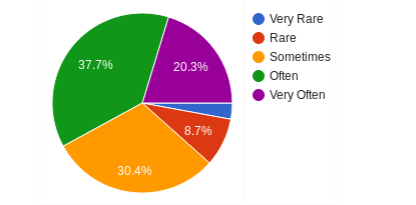
\includegraphics{Q1SE}
\caption{Concept Discussion with friends.}
\end{figure}

The data represented that 58 percent students discussed concepts and problems with their friends, with additional 30.4 percent discussing sometimes. It is symbolic of the fact that collaborative learning is indeed a great tool to improve the overall learning process. 

\textbf {2. Did you ever need help in understanding some core concepts and specific problems?}

\begin{figure}[ht]
\centering
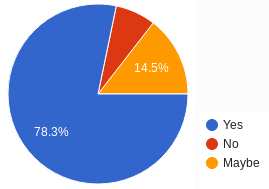
\includegraphics{Q2SE}
\caption{Need help in Understanding core concepts.}
\end{figure}

With 78.3 percent students needing help in the learning of concepts, it becomes clear that peer-to-peer tutoring would be in demand and with right approach and execution. 

\textbf {3. Do you often go to TA for help during the semester?}
\begin{figure}[ht]
\centering
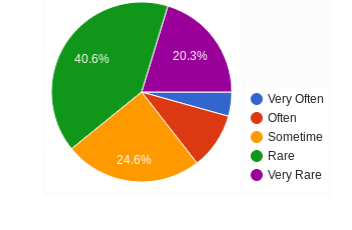
\includegraphics{Q3SE}
\caption{Concept Discussion with friends.}
\end{figure}

In the survey, 60.3 percent students responded that they do not to TA for seeking help. That shows that in spite of university providing excellent resources to cater to student needs, there is some gap between what is expected and what is offered. Or, there might just be the general mentality to avoid dealing with TAs since they have the control over students grades. Hence, the system calls for additional resources and not replacing existing ones. 

\textbf {4. Would you trust a fellow NC State student to tutor you in their field of expertise (based on peer reviews).}
\begin{figure}[ht]
\centering
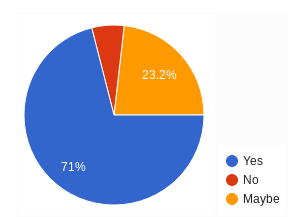
\includegraphics{Q4SE}
\caption{Trusting Fellow Students.}
\end{figure}

With 71 percent students accepting the idea of being tutored by their fellow students, it shows the great potential for the expansion and execution of the idea. Also, it is a validation based system hence only NCSU students can sign up to be tutors or to be tutored. University affiliation also gives a sense of confidentiality since both the parties are connected to the university and appropriate actions can be taken on violation of any policies. 

\textbf {5. Are you willing to tutor fellow NC State students in your free time?}
\begin{figure}[ht]
\centering
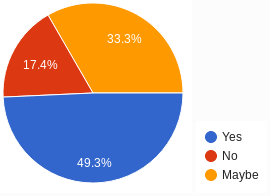
\includegraphics{Q5SE}
\caption{Willing to tutor.}
\end{figure}

Even if 49.3 percent of the students agree to tutor, we can have a very good population of tutors available at all times. Only 17.4 percent students denied to tutor and hence with correct marketing and execution, we can have a very good population of tutor community.

\textbf {6. Will you do tutoring free or only if being paid?}
\begin{figure}[ht]
\centering
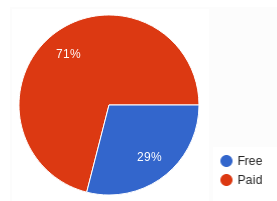
\includegraphics{Q6SE}
\caption{Paid Vs Free Tutoring.}
\end{figure}
Majority of the students, 71 percent expect some kind of payment for their tutoring efforts, which is only fair. Hence, we plan to integrate some rewards system wherein tutors can gain tangible rewards for their efforts like coupons or cash.

\section{Features}
In this section, we propose some of the key features of our application which we are planning to implement throughout our development cycle.


\subsection{Tutor-Student Matching}
A student signup and set up a profile where he provides information on which subjects he/she needs help in and which topic specifically on that subject. Based on the input, the system will use a searching algorithm for tutors based on the reviews and rating. The student can then select one from them according to his/her preference. The students can also look at the profile of the tutor and will also have the option to select paid tutor or a free tutor.

\subsection{Scheduling Tutoring Session}
Tutors will upload their preferred tutoring timing. Once the student selects a tutor, that tutors available timing will be displayed to the user. The user needs to select one of the timings which is convenient for both and an appointment will be scheduled. An email notification will be sent to both and the event will be added to both calendars.
\linebreak
\subsection{Reviews and Rating}
At the end of a tutoring session, the student needs to rate and give a review to the tutor. This rating and review will help other students in searching a good tutor for help and it will also help the tutors in adjusting their points that they will charge in each session. 

\subsection{Reward System}
On sign up, each user will receive some points which they can use to get the tutor. To learn or get help from someone, the student needs to spend points for that or he can get a free tutor. The tutor will earn the points that he has set for each session with the student. The tutor can also covert these points into gift vouchers. Based on the rating and reviews, a tutor can increase or decrease points for a tutoring session.

\section{Architecture}
\begin{figure}[ht]
\centering
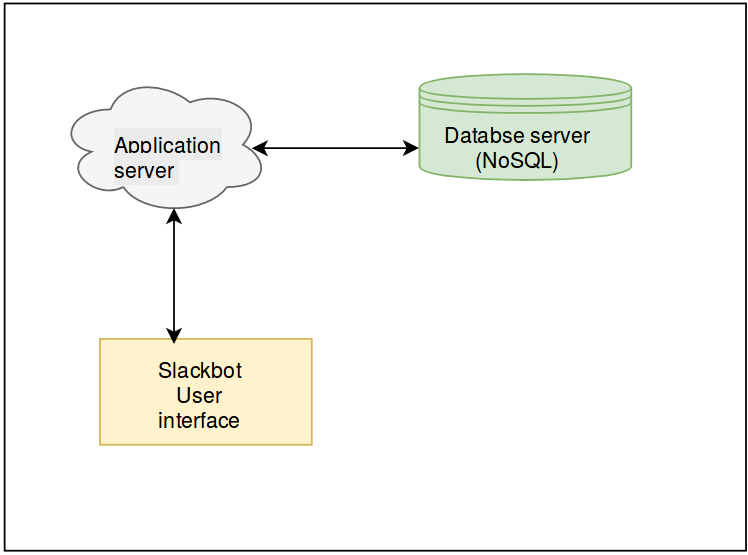
\includegraphics[width=85mm]{pic.png}
\caption{Architecture of the project}
\end{figure}

\subsection{User Interface}
For the user interface we will be using the slack user interface. So, the user will be sending the input as chat messages and our application server will process the request and display the output on the same page. The main advantage of this is that the user will find it user friendly and the user do not need to learn and understand the application to use it.

\subsection{Application server}
Application server will be developed using NodeJS which will communicate with the front-end module (slack-bot to process user queries. The queries that would be supported are find a tutor, arrange a meeting, review a tutor, etc. The data related to those will be stored in the database. The application server would be where the business logic resides. It will be the point of communication between the sla

\subsection{Database server}
For storing the data we will be using the no SQL database where we will be storing the information about tutors, meetings and transactions.



\section{Evaluation}

We propose four different methodologies for solving the peer to peer tutoring problem. The first approach is the traditional approach in which there is a tutoring center where a tutor is available and the students can go there and he can get help. If the tutor is not available then an official can schedule the student when the tutor is available. The second methodology is a scheduling mechanism where the tutor and students are registered to our platform and the students can book the tutor and they can schedule the time and place to meet. The third methodology is an on-demand mechanism where the students can request the topic for which the help is needed.  The tutors will see the requests and will try to serve the requests. If someone has requested a similar video before then the students can watch that video immediately. The fourth methodology is a real-time mechanism in which we will have an online platform where the students can get help in real-time. In this methodology, the students can select the tutor who is available and a real-time session will be created between the tutor and the students.

\begin{table}[ht]
\centering
\caption{Evaluation of Different Methodology}
\begin{tabular}{|c|c|c|c|c|c|1|} \hline
Methodology&1&2&3&4&5&6\\ \hline
Traditional &-&+&+&++&-&- -\\ \hline
Scheduled &++&++&-&+&+&+\\ \hline
On-Demand &-&- -&++&- -&- -&++\\ \hline
Real-Time &-&++&++&+&++&- -\\ \hline
\end{tabular}
\end{table}

\subsection{Evaluation Analysis}
We have evaluated the above mentioned four approaches based on various factors like Predictability(1), Availability(2), Security(3), Adaptability(4), Speed(5), Cost(6).
\linebreak
\subsubsection{Predictability}

In the traditional approach there is less predictability because the tutoring center cannot predict when a student will come to get tutored, this even holds true for the real-time methodology. The scheduled approach works best for predictability because there is a prior meeting booked so both the tutor and the student can predict when they will meet. For the on-demand methodology, we cannot predict when will the video be available.

\subsubsection{Availability}

 In the traditional methodology, tutors would be available only during the time of tutoring hours and not based on the availability of the student. For the Scheduled methodology, tutors will be available on the time decided by the tutor and the student.  For on-demand, the availability of the video can be instantaneous or it can even take days to get the answer and for real-time tutor can be available 24*7.

\subsubsection{Security}

We believe that the real-time and on-Demand methodology will be the most secure as there is no contact between the tutor and the student. Even the traditional methodology will be secure as it will the tutoring will happen in the secured designated area. The scheduled methodology can be less secure if the tutor and the student plan to meet outside the premises of university but to increase the security of the Scheduled Methodology one possible solution is to have the scheduled sessions only at the library.

\subsubsection{Adaptability}

According to our analysis, we think that student would easily adapt the traditional methodology as this approach is not something new and is tested and proven. The scheduled approach is also easy to adapt as the student always like to set meetings with their teams and friends to discuss the concepts. The on-demand approach might not be easy to adapt because if the video is not available the user might have to wait for some time until someone creates a video for him. Students might not adapt to this approach well because they do not like to wait without an estimated time period.  The real-time approach will be adapted well as its very easy and convenient for the students.

\subsubsection{Speed}

The real-time methodology would be the fastest as the student can get help anytime he wants whereas the on-demand can be the worst in terms of speed if the video is not found. The traditional is not that fast as the student cannot get help if the tutoring center is closed(eg. weekends). The scheduled methodology can be fast as the student can see the tutors availability and can book him for that time.

\subsubsection{Cost}

The real-time methodology will be the most costly as we will need to have a tutor always available. The traditional methodology will also be costly as the tutor will come to the tutoring center irrespective of the student being there or not. The Scheduled methodology will be cheaper as the tutor only gets paid for the hours that he tutors. The on-demand will be the cheapest as the tutor only creates video and gets paid when there is a request from the student.


\section{Conclusion}

%\end{document}  % This is where a 'short' article might terminate
Peer tutoring is not remedial but it is supplemental. Multiple research suggests that peer tutoring is very effective and sometimes it is twice powerful as learning. Multiple universities have their own university peer tutoring program. NC State has a peer tutoring system which is very limited and an offline process. We aim to provide a platform for peer tutoring such that all students of NC State can take the advantage. Also, WolfTutor is designed keeping campuses and students in mind for security and safety concerns.
%
% The following two commands are all you need in the
% initial runs of your .tex file to
% produce the bibliography for the citations in your paper.
\bibliographystyle{abbrv}
\bibliography{sigproc}  % sigproc.bib is the name of the Bibliography in this case
% You must have a proper ".bib" file
%  and remember to run:
% latex bibtex latex latex
% to resolve all references
\end{document}
